\section{Population Generation}

When the terrain has been generated, the PopulationGenerator commences a visual tool for the user to place a city marker.
When one or more markers are placed, the road generation begins immediately after pressing the generate roads button. 

Roads and highways will tend towards densely populated areas, and the size of buildings will vary depending on how intense the density is.

\begin{figure}[h!]
  \centering

  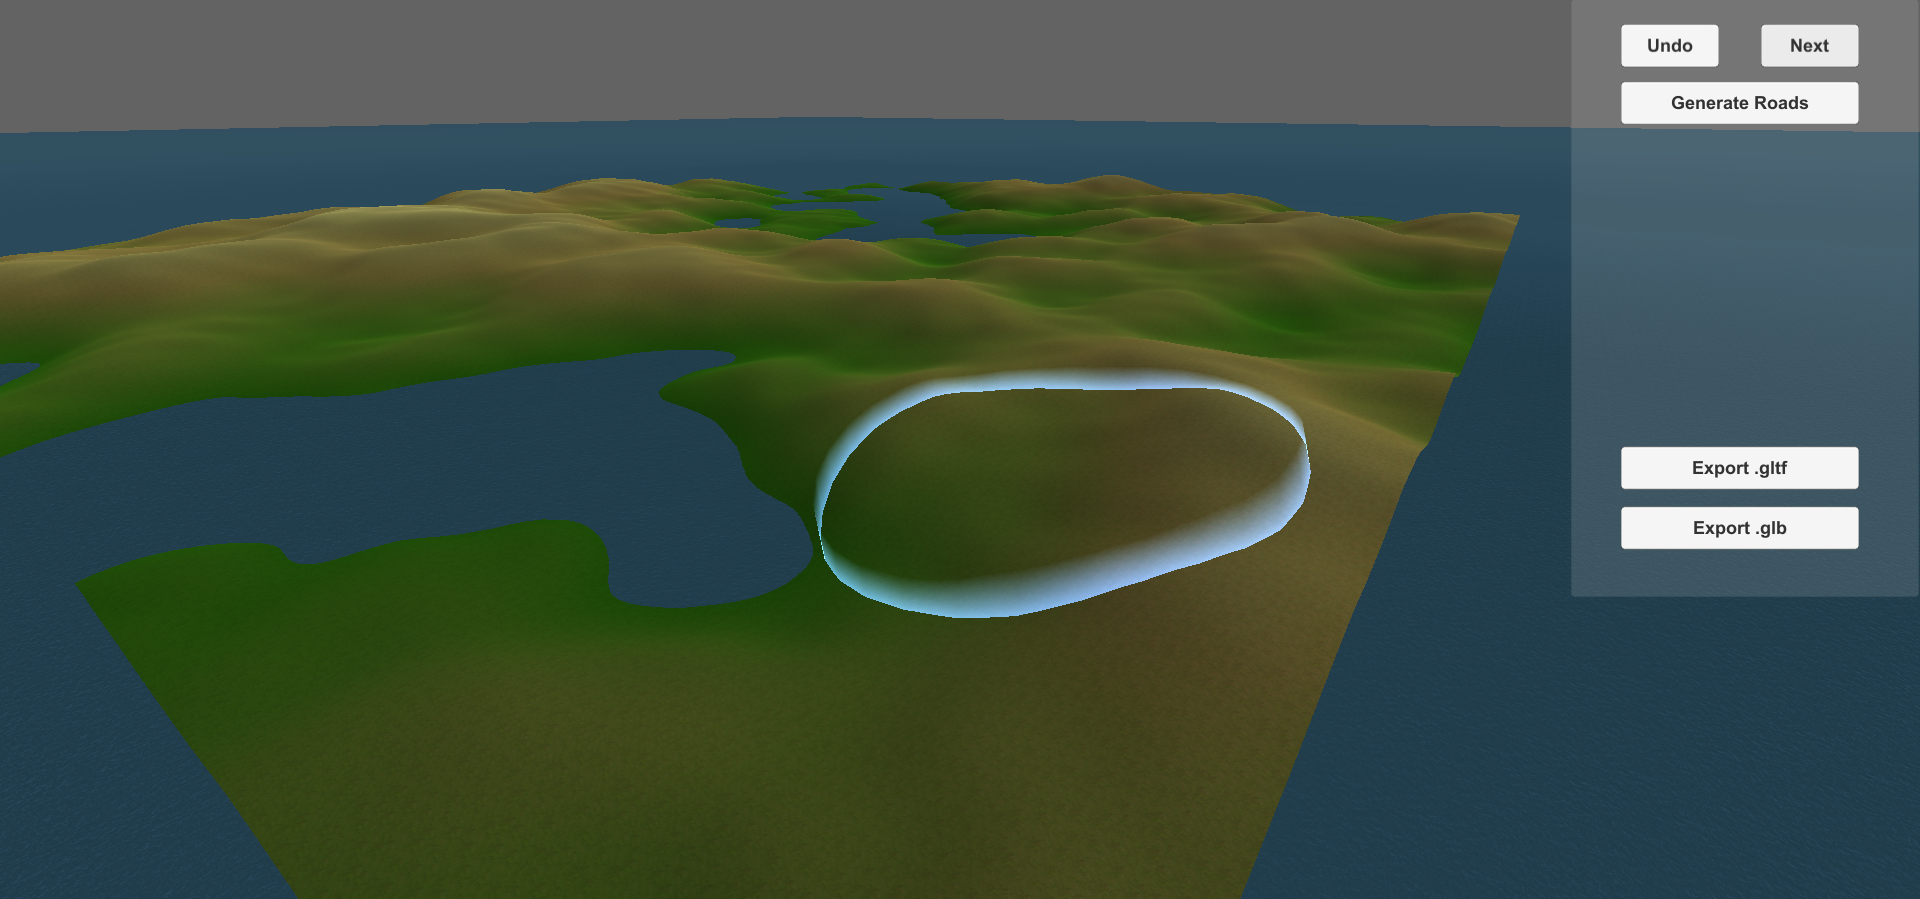
\includegraphics[width=0.8\textwidth]{figure/city_marker_tool.png}
  \caption{The city marker tool visuals.}

  \label{fig:citymarker}
\end{figure}